\documentclass[a4paper,12pt]{report}

\usepackage[utf8]{inputenc}
\usepackage{t1enc}
\usepackage[T1]{fontenc}
\usepackage[magyar]{babel}
\usepackage{indentfirst}
\usepackage{anysize}
\usepackage{graphicx}
\usepackage{wrapfig}
\usepackage{sidecap}
\usepackage{subfigure}
\usepackage{amsmath, amssymb, amsfonts}
\usepackage{latexsym}
\usepackage{todonotes}
\setlength{\parindent}{0pt}
\setlength{\parskip}{1ex plus 0.5ex minus 0.2ex}
\reversemarginpar
\setlength{\marginparwidth}{2.5cm}

\newtheorem{Tet}{Tétel}[section]
\newtheorem{Lem}[Tet]{Lemma}
\newtheorem{All}[Tet]{Állítás}
\newtheorem{Kov}[Tet]{Következmény}
\newtheorem{Def}[Tet]{Definíció}
\newtheorem{Megj}[Tet]{Megjegyzés}
\newtheorem{Jel}[Tet]{Jelölés}
\newtheorem{Pl}[Tet]{Példa}
\newtheorem{Fel}[Tet]{Feladat}
\newenvironment{Mo}{\noindent \textbf{Megoldás. }}{ $\clubsuit$}
\newenvironment{Biz}{\noindent \textbf{Bizonyítás. }}{ $\square$}

\newcommand{\noun}[1]{\textsc{#1}}
\newcommand{\blankpage}{
	\newpage
	\setcounter{page}{1}
	\thispagestyle{empty}
	\mbox{}
	\newpage
}
\newcommand{\todored}[1]{\todo[color=red!70, size=\footnotesize]{#1}}
\newcommand{\todoor}[1]{\todo[color=orange!90, size=\footnotesize]{#1}}

\begin{document}




% Első három oldal:



	\thispagestyle{empty}
	\begin{center}
		{\large \noun{Eötvös Lóránd Tudományegyetem \\ Természettudományi Kar} }
		\line(1,0){455}
		\vspace{80pt}
		{\Huge \noun{\textbf{Véletlen iterációk statisztikai elemzése}}}
		\vspace{20pt}
		\\BSc Szakdolgozat
		\vspace{90pt}
		\\Írta: Mészáros Ádám István\\ Matematika BSc, Matematikai elemző szakirány\\
		\vspace{35pt}
		Témavezető: Sigray István\\ Műszaki Gazdasági Tanár, Analízis tanszék\\
		\vspace{80pt}
		
\includegraphics[scale=0.21]{elte.png}
		\vspace{25pt}
		\\ 2013\\ Budapest
	\end{center}
	\blankpage
	\tableofcontents



%%=========================================================================================
%%========================== szakdolgozat tartalmi része ==================================
%%=========================================================================================


	%%%%%%%%%%%%%%%%%%%%%%%%%%%%%%%%%%%%%%%%%%%%%
	%				1. FEJEZET
	%				BEVEZETÉS
	%%%%%%%%%%%%%%%%%%%%%%%%%%%%%%%%%%%%%%%%%%%%

	\chapter{Bevezetés}
		Lorem ipsum dolor sit amet, consectetur adipisicing elit, sed do eiusmod tempor incididunt ut labore et dolore magna aliqua. Ut enim ad minim veniam, quis nostrud exercitation ullamco laboris nisi ut aliquip ex ea commodo consequat. Duis aute irure dolor in reprehenderit in voluptate velit esse cillum dolore eu fugiat nulla pariatur. Excepteur sint occaecat cupidatat non proident, sunt in culpa qui officia deserunt mollit anim id est laborum.
	
	%%%%%%%%%%%%%%%%%%%%%%%%%%%%%%%%%%%%%%%%%%%%%
	%				2. FEJEZET
	%				A NEWTON-MÓDSZER
	%%%%%%%%%%%%%%%%%%%%%%%%%%%%%%%%%%%%%%%%%%%%
	
	\chapter{A Newton-módszer}
    
    
    	%
        %	2.1 módszer leírása
        %
        
        
		\section{A módszer leírása}
        	\todoor{Változtatás: A bevezető szövegben egy kis átírás. Nekem kevésbé tűnik eröltetettnek.}
			A Newton-módszer, mint a neve is mutatja, először Isaac Newton dolgozta ki, azonban a mai formáját Joseph Raphson írta le 1690-ben %Raphson, J. Analysis aequationum universalis. London, 1690. 
            , ezért Newton-Raphson-módszernek is hívják. Newton a módszert eredetileg polinomokra alkalmazta, ahogy a későbbiekben majd én is teszem.\\ A Newton-módszer egy iterációs eljárás nemlineáris egyenletek gyökeinek megtalálására, közelítésére. A módszer - valós esetben - egy geometriailag nagyon egyszerű meggondoláson alapul, amit egy kép segítségével fogok bemutatni.
			\begin{figure}[htp]
				\centering
				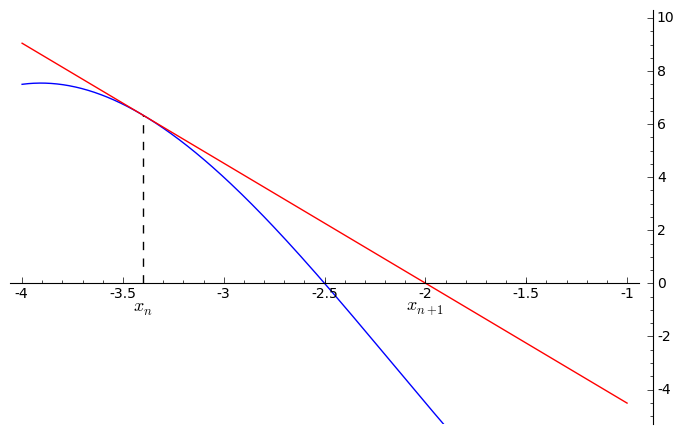
\includegraphics[scale=0.5]{kep1.png}
				\caption{Egy lépés a Newton-módszerrel}\label{k1}
			\end{figure}
			Első lépésként vegyünk egy kezdőpontot az $x$ tengelyen, amely elég közel van a gyökünkhöz. Jelöljük $x_0$-lal. Tegyük fel, hogy $n$ lépés után eljutottunk az $x_n$ pontig. Húzzunk érintőt a grafikonhoz ebben a pontban. Az érintő és az $x$ tengely metszéspontja legyen a következő pontunk, $x_{n+1}$, majd így folytassuk amíg elég közel nem kerülünk a egyenletünk gyökéhez.
			\\ Tegyük fel, hogy $x_k$ közel van az $f(x)=0$ egyenlet $x^*$ gyökéhez, és $f$ kétszer folytonosan differenciálható. \todoor{Változtatás: következő mondat a Tanár úr megjegyzése alapján} Ekkor felírhatjuk $f$ Taylor-sorát maradéktaggal a következőképpen
			\[ f(x^*)=f(x_k)+f'(x_k)(x^*-x_{k})+O((x^*-x_{k})^2) \]
			$f(x^*)$ lineáris közelítéséhez nincsen szükségünk az $(x^*-x_{k})^2$-es tagokra.
			\begin{eqnarray*}
				f(x^*)&\approx& f(x_k)+f'(x_k)(x^*-x_{k})\\
				0&\approx&\frac{f(x_k)}{f'(x_k)}+(x^*-x_{k})\\
				x^*&\approx & x_k-\frac{f(x_k)}{f'(x_k)}
			\end{eqnarray*}
			Definiáljunk egy lépést a közelítés jobb oldalával, így előállíthatjuk a következő iterációt
			\begin{equation}
				 \label{e2} x_{k+1}=x_k-\frac{f(x_k)}{f'(x_k)}
			\end{equation}
			\begin{Pl}
				Az alábbiakban a \ref{k1} képen ábrázolt polinommal fogok számolni.
				\[f(x)=x^3+6.5x^2+5x-12.5\]
				$f(x)=0$ egyenletnek gyöke az $x^*=2.5$. Induljunk el az $x_0=-1$ pontból.
				\begin{center}				
					\begin{tabular}{|c|c|c|c|c|c|}
						\hline
						$k$ & $0$ & $1$ & $2$ & $3$ & $4$ \\
						\hline
						$x_k$ & $-1$ & $-3.4$ & $-1.9982$ & $-2.5001$ & $-2.5$ \\
						\hline
						$f(x_k)$ & $-12$ & $6.336$ & $-4.5159$ & $8.6664\cdot 10^{-4}$ & $-9.8121\cdot 10^{-9}$ \\
						\hline
						$|x_k-x^*|$ & $1.5$ & $0.9$ & $0.5018$ & $9.9045\cdot 10^{-5}$ & $1.1214\cdot 10^{-9}$ \\
						\hline
					\end{tabular}
				\end{center}
            \end{Pl}
            \todoor{Megjegyzés: Nem tudom, hogy a táblázatban hogyan tüntessem fel, hogy a negyedik lépésnél $x_k\approx-2.5$, de nem egyenlő, különben a másik két sor értékei hibásak. Sajnos a pontos érték nem fér ki a táblázatba.}
    	
        
        %
        %	2.2 konvrgencia vizsgálat
        %
        
        
		\section{Konvergencia vizsgálat}
			\todoor{Változtatás: A jelölés részt előrrébb hoztam, hogy a tételt precízebben ki tudjam mondani, és $m_1$, $M_2$ definícióit a Tanár úr megjegyzése alapján átírtam.}
            \begin{Jel}
				$m_1:=\smash{\displaystyle \min_{x \in [x_k,x^*]}} |f'(x)|$, $M_2:=\smash{\displaystyle \max_{x\in [x_k,x^*]}} |f''(x)|$, $C:=\frac{M_2}{2m_1}$
			\end{Jel}
			\begin{Tet}
			\label{t2} Tegyük fel, hogy $f\in C^2[a,b]$, és egyértelműen létezik $x^*\in [a,b]$ amelyre $f(x^*)=0$, továbbá $m_1>0$, és $M_2<\infty$. Ekkor, ha a Newton-módszer konvergens, akkor másodrendben konvergál a gyökhöz.
			\end{Tet}
			\begin{Biz}
				Fejtsük $f(x^*)$-ot Taylor-sorba $x_k$ körül, és írjuk ki a Lagrange-féle maradéktagot 
				\begin{eqnarray}
					f(x^*)&=&f(x_k)+f'(x_k)(x^*-x_{k})+\frac{f''(\xi)}{2}(x^*-x_{k})^2 \\
					0&=&\frac{f(x_k)}{f'(x_k)}+(x^*-x_{k})+\frac{\frac{f''(\xi)}{2}(x^*-x_{k})^2}{f'(x_k)}\\
					\label{e1} x^*&=&x_k-\frac{f(x_k)}{f'(x_k)}-\frac{f''(\xi)}{2f'(x_k)}(x^*-x_{k})^2
				\end{eqnarray}
				Ahol $\xi \in (x_k,x^*)$. Vonjuk ki a \ref{e2} egyenletből a \ref{e1}-t
				\begin{eqnarray*}
					x_{k+1}-x^*&=&\left(x_k-\frac{f(x_k)}{f'(x_k)}\right) - \left(x_k-\frac{f(x_k)}{f'(x_k)}-\frac{f''(\xi)}{2f'(x_k)}(x^*-x_{k})^2\right)\\
					x_{k+1}-x^*&=&\frac{f''(\xi)}{2f'(x_k)}(x^*-x_{k})^2\leq C |x^*-x_k|^2
				\end{eqnarray*}
				Vagyis a következőt kapjuk
				\begin{equation}
					\label{e3}|x_{k+1}-x^*|\leq C |x^*-x_k|^2
				\end{equation}
				Ez azt jelenti, hogyha a Newton-módszer konvergens, akkor másodrendben konvergál.
			\end{Biz}
			
			Hogyan tudjuk garantálni a konvergenciát? \todoor{Változtatás: Tanár úr megjegyzése alapján a következő mondat} \ref{e3} egyenlőtlenséget a következőképpen tudjuk iterálni $x^*$ közelében
			\begin{eqnarray}
				|x_k-x^*|&\leq& C |x^*-x_{k-1}|^2\\
				&\leq & C\left |C|x^*-x_{k-2}|^2\right |^2=C^3|x^*-x_{k-2}|^4\\
				&\leq & \ldots\leq C^{2^k-1} |x^*-x_0|^{2^k}\label{e4}			
			\end{eqnarray}
			Vagyis $|x_k-x^*|\leq C^{2^k-1}|x^*-x_0|^{2^k}$. Szeretnénk, ha a következő teljesülne
			\[ \lim_{k \to \infty} |x^*-x_k|=0\]
			Ha a \ref{e4}-as egyenletben az egyenlőtlenség jobb oldala tart nullához, akkor a Rendőr-elv alapján ez teljesül.
			\[ C^{2^k-1}|x^*-x_0|^{2^k}=q^{2^k-1}|x^*-x_0| \] 
			Ez akkor és csak akkor tart nullához, ha $q<1$.
			\[q=C|x^*-x_0|=  \frac{M_2}{2 m_1} \left |x^*-x_0 \right | < 1 \]
			Átrendezve
			\[ |x_0-x^*|<  \frac{2 m_1}{M_2} \]
			Ezek alapján a következő tételt mondhatjuk ki
			\todoor{Változtatás: beleírtam, hogy van egy $I$ intervallumunk, és $m_1$, $M_2$ definícióját átírtam erre az intervallumra. Úgy gondolom így áthidaltam azt a problémát, hogy eddig ezek a konstansok függtek $x_k$-tól. A 3. pontot átírtam $M_2$ jelölés felhasználásával.}
            \begin{Tet}
				Legyen $I$ egy adott intervallum, és $m_1:=\smash{\displaystyle \min_{x \in I}} |f'(x)|$, $M_2:=\smash{\displaystyle \max_{x\in I}} |f''(x)|$. Tegyük fel a következőket	
				\begin{enumerate}
					\item $f(x)$-hez $!\exists x^*\in I$, amire $f(x^*)=0$
					\item $f(x)$ kétszer folytonosan deriválható az $I$ intervallumon
					\item $M_2<\infty$
					\item $\forall x \in I$-re $f'(x) \neq 0$ 
					\item $x_0 \in \left (x^*-\frac{2 m_1}{M_2},x^*+\frac{2 m_1}{M_2}\right )$	
				\end{enumerate}
				Ekkor $\smash{\displaystyle \lim_{k\to \infty} }x_k= x^*$.
			\end{Tet}
            \todoor{Változtatás: A következő eddig megjegyzés környezetben volt}
			Ezeket sajnos elég nehéz garantálni. Például az 5. feltételhez tudnunk kell, hogy mi a gyök, aminek a meghatározására alkalmaznánk a módszert. A 4. feltétel ellenőrzése szintén bonyolult, hiszen ehhez először meg kellene határoznunk a derivált gyökeit, amivel szintén az eredeti problémához jutunk.
            \begin{Tet}
				\label{t1}
				Tegyük fel, hogy $f\in C^2[a,b]$, és egyértelműen létezik $x^*\in [a,b]$ amelyre $f(x^*)=0$, továbbá $x_0\in [a,b]$, $\forall x \in (x^*,x_0)$-re $f'(x)$,$f''(x) \neq 0$, és $x_0$-ra teljesül, hogy $f(x_0)f''(x_0)>0$, akkor $x_k$ szigorúan monoton tart a gyökhöz.
			\end{Tet}
            \todoor{Változtatás: A tétel feltételeit átírtam hasonló stílusúra mint amiket előzőekben már használtam}
			\begin{Biz}
				Négy esetünk van.
				\begin{enumerate}
					\item $x_0>x^*$, $f(x_0)>0$
					\item $x_0>x^*$, $f(x_0)<0$
					\item $x_0<x^*$, $f(x_0)>0$
					\item $x_0<x^*$, $f(x_0)<0$
				\end{enumerate}	
				Az esetek bizonyítása nagyban hasonlít, ezért csak az elsőt látjuk be. Mivel $f(x_0)>0$ és $f(x_0)f''(x_0)>0$, ezért $f''(x_0)>0$. Továbbá $(x^*,x_0)$-n $f'(x)\neq 0$, ezért az vagy mindenhol pozitív, vagy mindenhol negatív. 
				\begin{eqnarray}
					\label{e6}0&<&f(x_0)\\
					\label{e7}&=&f(x_0)-f(x^*)\\
					\label{e8}&=&f'(\xi)\underbrace{(x_0-x^*)}_{>0}
				\end{eqnarray}
				\ref{e7} $\Rightarrow$ \ref{e8} a Lagrange-féle középérték tétel miatt, valamilyen $\xi \in (x^*,x_0)$-re. Ez azt jelenti, hogy $f'(\xi)>0$, amiből következik, hogy $\forall x\in (x^*,x_0): f'(x)>0$. Ez alapján a következőt tudjuk
				\begin{eqnarray*}
					x_{k+1}&=&x_k-\underbrace{\frac{f(x_k)}{f'(x_k)}}_{>0} \\
					x_{k+1}&<&x_k
				\end{eqnarray*}
				Vagyis az $x_k$ sorozat szigorúan monoton csökkenő. Használjuk ismét a Lagrange-féle középérték tételt
				\[0<f(x_k)=f(x_k)-f(x^*)=\underbrace{f'(\xi)}_{>0}(x_k-x^*)\]
				Tehát $x_k>x^*$ azaz $x_k$ sorozat korlátos. A korlátosságból, és a monotonitásból következik, hogy $x_k$ konvergens. Tegyük fel, hogy $x_k\to \tilde{x}^*$.
				\begin{eqnarray*}
					\lim_{k \to \infty} x_{k+1} &=& \lim_{k \to \infty} x_k - \dfrac{\lim\limits_{k \to \infty} f(x_k)}{\lim\limits_{k \to \infty} f'(x_k)}\\
					\tilde{x}^*&=&\tilde{x}^*-\dfrac{f(\tilde{x}^*)}{f'(\tilde{x}^*)}\\
					\dfrac{f(\tilde{x}^*)}{f'(\tilde{x}^*)}&=&0
				\end{eqnarray*}
				Ez csak akkor lehetséges, ha $f(\tilde{x}^*)=0$, viszont $x^*$ gyök egyértelmű, ezért $x^*=\tilde{x}^*$.
			\end{Biz}
            
            
    	%
        %	2.3 Leállási feltétel
        %
            
            
		\section{Leállási feltétel}
			\begin{Jel}
				$m_1:=\smash{\displaystyle \min_{x \in (a,b)} } \left| \left( \dfrac{f(x)}{f'(x)} \right)' \right|$
			\end{Jel}
			\begin{Tet}
				Tegyük fel, hogy $f\in C^2[a,b]$ és $m_1>0$. Ekkor ha valamilyen $\varepsilon >0 $-ra és k indexre
				\begin{equation}
					\label{e5} \left| \frac{x_{k+1}-x_k}{x_k} \right |\leq \frac{\varepsilon}{\varepsilon+1}m_1
				\end{equation}
				akkor $|x_k-x^*|\leq \varepsilon|x^*|$.
			\end{Tet}
			\begin{Biz}
				Rendezzük át a \ref{e2} egyenletet és alkalmazzuk a Lagrange-féle középérték tételt.
				\begin{eqnarray*}
					| x_{k+1} - x_{k}|&=& \left| \frac{f(x_k)}{f'(x_k)} \right| \\
					&=& \left| \frac{f(x_k)}{f'(x_k)}- \frac{f(x^*)}{f'(x^*)} \right| \\
					&=&\left| \left(\frac{f(\xi)}{f'(\xi)}\right)'\right| \cdot |x_k-x^*|
				\end{eqnarray*}			
				ahol $\xi \in (x*,x_k)$
				\[| x_{k+1} - x_{k}|\geq m_1 |x_k-x^*| \]
				Fejezzük ki \ref{e5} -t $m_1$-re és helyettesítsük be.
				\begin{eqnarray*}
					| x_{k+1} - x_{k}|&\geq& \frac{|x_{k+1}-x_k|}{|x_k|}\cdot \frac{\varepsilon+1}{\varepsilon}\cdot |x_k-x^*|\\
					\varepsilon |x_k|&\geq& \varepsilon  |x_k-x^*| + |x_k-x^*|\\
					 |x_k-x^*|&\leq &\varepsilon (|x_k|- |x_k-x^*|)\\
					&\leq& \varepsilon(|x_k-x_k+x^*|)=\varepsilon |x^*|
				\end{eqnarray*}
			\end{Biz}
			\begin{Kov}
				Tegyük fel, hogy szeretnénk $e$-nél kisebb hibával közelíteni $x^*$-ot. Mivel $|x^*|\leq\max \{ |a|,|b| \}$, ha ismerünk, egy olyan $\varepsilon$ számot, amelyre teljesül a tételbeli feltétel, és $\varepsilon \max \{|a|,|b|\} \leq e$, akkor
				\[ |x_k-x^*|\leq \varepsilon |x^*| \leq \varepsilon \max \{|a|,|b|\} \leq e \]
			\end{Kov}
			\todoor{Változtatás: Innentől kezdve minden új}
			Sajnos ez a leállási feltétel nem túl hasznos, hiszen minden lépésnél újabb $\varepsilon$-t kell keresnünk, ami műveletigényes.



    	%
        %	2.4 Komplex eset
        %

		\section{Komplex eset}
			Érdemes megvizsgálni a módszert komplex gyökkel rendelkező egyenletekre is. Ekkor a fentiekkel analóg állítások mondhatók ki. A komplex eset geometriai meggondolása is hasonló. $z=x+yi\in \mathbb{C}$. Vegyük a $|f(z)|$ függvényt. Ekkor $z_{k+1}$ az a $z_k$-hoz legközelebbi pont amely a komplex sík és az $|f(z)|$ függvény $z_k$ pontban vett érintő síkja metszésvonalán helyezkedik el (\ref{k6}). Meggondolható, hogy ez valós esetben ugyanazt jelenti mint eddig, hiszen a két sík metszésvonala helyett, az x tengely és az érintő egyenes metszéspontját vesszük. A lépés iránya ezáltal ellentétes $|f(z)|$ gradiensével a $z_k$ pontban. \cite{Yau98}
            \begin{figure}[htp]
				\begin{center}
				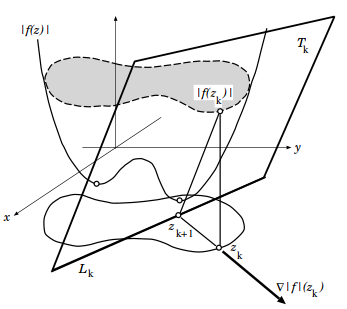
\includegraphics[scale=0.6]{kep6.png}
				\caption{A komplex eset geometriai meggondolása \cite{Yau98}} \label{k6}
				\end{center}
			\end{figure}
            
            Vegyük például a $f(x)=x^2-2i$ komplex együtthatós polinomot, amelynek az $1+i$ és a $-1-i$ a gyökei. A gradiensnél (\ref{k7}) valamivel jobb szemléltetés végett definiáljuk a következő vektormezőt
			\[g(x,y)=\left(\mathrm{Re} \left\{ -\frac{f(x+yi)}{f'(x+yi)} \right \} ,\mathrm{Im} \left\{-\frac{f(x+yi)}{f'(x+yi)}\right \} \right)\]
			
			Ezt ábrázolva láthatjuk, hogy az esetünkben hogyan fog haladni a komplex síkon a módszer. A \ref{k4} ábrán jelöltem $1-0.5i$-ből indított módszer pontjait is. A kezdőpont pirossal van ábrázolva, ami az iterációs lépésekkel átvált sárgába.
			
            \begin{figure}[htp]
           		\hfill
           		\subfigure[$-\operatorname{grad}\,|f(z)|$ szintvonalai]{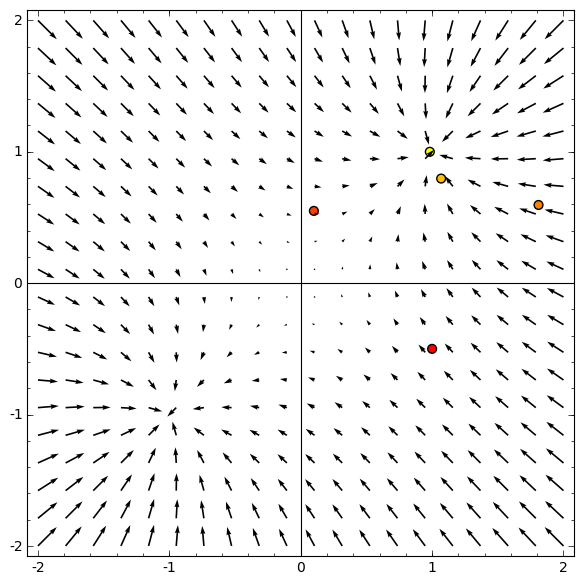
\includegraphics[scale=0.5]{kep7.png} \label{k7}}
           		\hfill
            	\subfigure[$g(x,y)$ és négy iterációs lépés az $1-0.5i$-ből]{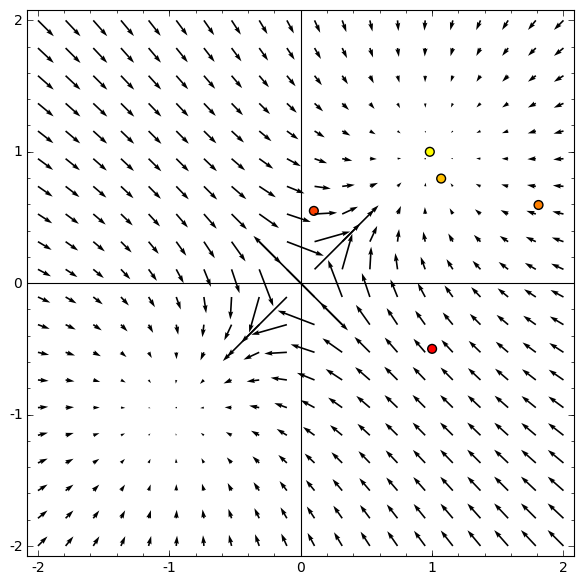
\includegraphics[scale=0.5]{kep4.png} \label{k4}}
            	\hfill
           	 	\caption{A komplex eset szemléltetése} 
           	\end{figure}
            \begin{Pl}
				\ref{k4} számokkal
				\begin{center}				
					\begin{tabular}{|c|c|c|c|c|c|}
						\hline
						$k$ & $0$ & $1$ & $2$ & $4$ & $4$ \\
						\hline
						$z_k$ & $1-0.5i$ & $0.1+0.55i$ & $0.81+0.595i$ & $1.069+0.796i$ & $0.983+i$ \\
						\hline
						$|f(z_k)|$ & $3.092$ & $1.912$ & $2.926$ & $0.59$ & $0.049$ \\
						\hline
						$|z_k-z^*|$ & $1.5$ & $1.006$ & $0.906$ & $0.215$ & $0.017$ \\
						\hline
					\end{tabular}
				\end{center}
            \end{Pl}
			Láthatjuk, a módszer nem csak komplex gyökökkel rendelkező valós polinomokra működik, de komplex együtthatós polinomokra is. Azonban ha egy valós polinom komplex gyökét szeretnénk meghatározni, akkor szükséges, hogy a kezdőpontunk képzetes része eltérjen nullától, különben az iterációs lépés tulajdonásága miatt $\forall z_k\in \mathbb{R}$.
            
            \begin{figure}[htp]
				\begin{center}
				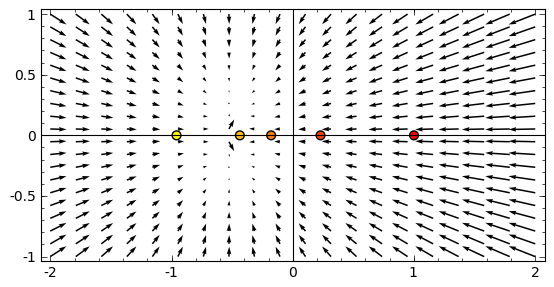
\includegraphics[scale=0.62]{kep5.png}
				\caption{$x^2 + x + 0.3125$ komplex gyökeinek keresése valós kezdőpontból} \label{k5}
				\end{center}
			\end{figure}




	%%%%%%%%%%%%%%%%%%%%%%%%%%%%%%%%%%%%%%%%%%%%%
	%				3. FEJEZET
	%				MÓDOSÍTOTT MÓDSZER POLINOMOKRA
	%%%%%%%%%%%%%%%%%%%%%%%%%%%%%%%%%%%%%%%%%%%%
    
    
    
	\chapter{Módosított módszer polinomokra}
    \todoor{Megjegyzés: Ez a fejezet még csak vázlat. Egyenlőre próbáltam összeírni valamilyen motivációt ami miatt módosítjuk a Newton-módszert.}
		Adott a Newton-módszer, amit az előző fejezetben vizsgáltunk. Tudjuk, hogyha az $x_k$ sorozat konvergens, akkor másodrendben konvergál a gyökhöz (\ref{t2}), sőt bizonyos feltételeket biztosítva monoton konvergenciát tudtunk biztosítani (\ref{t1}). Azonban sok esetben a módszer nem konvergens. Szeretnénk egy olyan módszert, amely viszonylag gyorsan és sok helyről konvergens.
		\section{Motiváció}
						Vizsgáljuk meg, hogy egy polinom hogyan viselkedik a \ref{t1} tétel alapján, vagyis honnan indulva garantált a monoton konvergencia.
			\begin{figure}[htp]
				\centering
				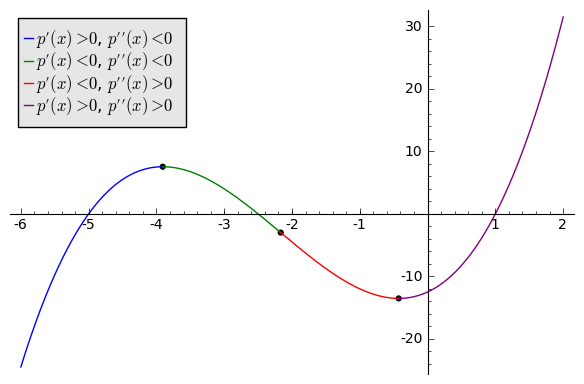
\includegraphics[scale=0.6]{kep2.png}
				\caption{Egy polinom felosztása az első és második deriváltjának viselkedése alapján}\label{k2}
			\end{figure}
			A tétel feltételei alapján a kezdőpontunk és a gyök közötti intervallumon sem a függvény deriváltja, sem a második deriváltja nem lehet nulla. Ez négy lehetőséget ad melyet a \ref{k2} ábrán szemléltettem. Mint az ábrán is látható előfordulhat olyan eset amikor egy ilyen intervallumon nincsen gyöke a polinomnak. Azonban amelyik intervallumon van, ott vagy a gyök előtti, vagy utáni részről véve a kezdőpontunkat a feltételek teljesülnek.
			\begin{figure}[htp]
				\centering
				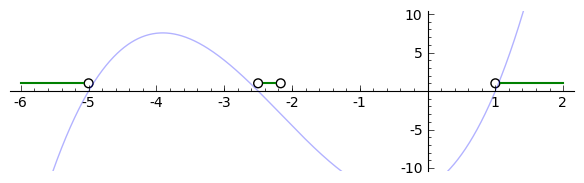
\includegraphics[scale=0.6]{kep3.png}
				\caption{Megfelelő intervallumok a kezdőpont választáshoz \ref{t1} tétel alapján}\label{k3}
			\end{figure}
			Láthatjuk, hogy esetünkben a kezdőpontunknak alkalmas intervallum majdnem lefedi a számegyenest, pont a gyökök közelében kimaradnak kisebb részek, és bár monoton és másodrendű konvergencia garantált például a két szélső intervallumban, ha távolról indulunk, előfordulhat hogy lassú lesz a módszer. További gondot jelenthet, ha a polinomnak komplex gyökei is vannak. 
			
			Ha egy polinomot leosztunk egy másik polinommal, és a két polinomnak nem egyezik meg valamelyik gyöke, akkor egy olyan függvényt kapunk amelynek a gyökei megegyeznek az eredeti polinomunkéval. Ugyanis legyen $p_1(x)$ a polinomunk amelyiknek a gyökeit keressük, és osszuk le $p_2(x)$ polinommal. Legyen $x^*$ gyöke $p_1(x)$-nek. Ekkor
			\[ \frac{p_1(x^*)}{p_2(x^*)}=\frac{0}{p_2(x^*)}=0\]
			
			Felvetődik tehát az ötlet, hogy hajtsuk végre a Newton-módszert a $\frac{p_1(x)}{p_2(x)}$ egyenlet gyökeinek keresésére. Vegyük azt a speciális esetet amikor $p_2(x)=p_1'(x)$. Ha $p_1(x)$-nek nincs többszörös gyöke, akkor a módosított egyenletünknek ugyanazok a gyökei.
			\begin{figure}[htp]
           		\hfill
           		\subfigure[Egy polinom és a módosított egyenlete]{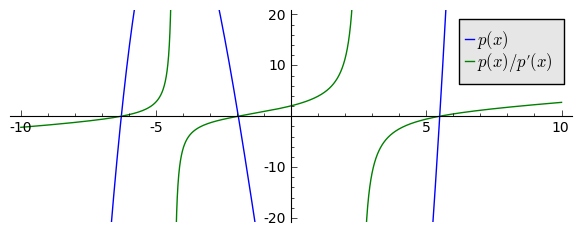
\includegraphics[scale=0.5]{sage8.png} \label{k8}}
           		\hfill
            	\subfigure[Megfelelő intervallumok a kezdőpont választáshoz \ref{t1} tétel alapján]{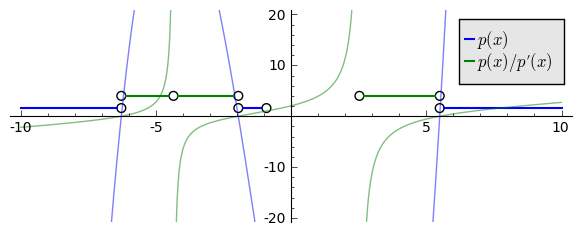
\includegraphics[scale=0.5]{sage9.png} \label{k9}}
            	\hfill
                \caption{}
           	\end{figure}
			
            Ahogyan \ref{k9}-en látható
% irodalomjegyzék
	\begin{thebibliography}{99}
		\bibitem{Yau98} Lily Yau and Adi Ben-Israel ``The Newton and Halley Methods for Complex Roots", \emph{The American Mathematical Monthly} Vol. 105, No. 9, November 1998 % http://folk.uib.no/ssu029/Pdf_file/Yau98.pdf

	\end{thebibliography}
\end{document}